%%%%%%%%%%%%%%%%%%%%%%%%%%%%%%%%%%%%%%%%%%%%%%%%%%%%%%%%%%%%%%%%%%%%%
%% This is a (brief) model paper using the achemso class
%% The document class accepts keyval options, which should include
%% the target journal and optionally the manuscript type. 
%%%%%%%%%%%%%%%%%%%%%%%%%%%%%%%%%%%%%%%%%%%%%%%%%%%%%%%%%%%%%%%%%%%%%
\documentclass[journal=jacsat,manuscript=article]{achemso}

%%%%%%%%%%%%%%%%%%%%%%%%%%%%%%%%%%%%%%%%%%%%%%%%%%%%%%%%%%%%%%%%%%%%%
%% Place any additional packages needed here.  Only include packages
%% which are essential, to avoid problems later. Do NOT use any
%% packages which require e-TeX (for example etoolbox): the e-TeX
%% extensions are not currently available on the ACS conversion
%% servers.
%%%%%%%%%%%%%%%%%%%%%%%%%%%%%%%%%%%%%%%%%%%%%%%%%%%%%%%%%%%%%%%%%%%%%
\usepackage[version=3]{mhchem} % Formula subscripts using \ce{}
\usepackage{algorithm}
\usepackage{algpseudocode}
\usepackage{svg}
\usepackage{amsmath}
\usepackage{hyperref}

%%%%%%%%%%%%%%%%%%%%%%%%%%%%%%%%%%%%%%%%%%%%%%%%%%%%%%%%%%%%%%%%%%%%%https://www.overleaf.com/project/63f3627b7f8554c152639004
%% If issues arise when submitting your manuscript, you may want to
%% un-comment the next line.  This provides information on the
%% version of every file you have used.
%%%%%%%%%%%%%%%%%%%%%%%%%%%%%%%%%%%%%%%%%%%%%%%%%%%%%%%%%%%%%%%%%%%%%
%%\listfiles

%%%%%%%%%%%%%%%%%%%%%%%%%%%%%%%%%%%%%%%%%%%%%%%%%%%%%%%%%%%%%%%%%%%%%
%% Place any additional macros here.  Please use \newcommand* where
%% possible, and avoid layout-changing macros (which are not used
%% when typesetting).
%%%%%%%%%%%%%%%%%%%%%%%%%%%%%%%%%%%%%%%%%%%%%%%%%%%%%%%%%%%%%%%%%%%%%
\newcommand*\mycommand[1]{\texttt{\emph{#1}}}

%%%%%%%%%%%%%%%%%%%%%%%%%%%%%%%%%%%%%%%%%%%%%%%%%%%%%%%%%%%%%%%%%%%%%
%% Meta-data block
%% ---------------
%% Each author should be given as a separate \author command.
%%
%% Corresponding authors should have an e-mail given after the author
%% name as an \email command. Phone and fax numbers can be given
%% using \phone and \fax, respectively; this information is optional.
%%
%% The affiliation of authors is given after the authors; each
%% \affiliation command applies to all preceding authors not already
%% assigned an affiliation.
%%
%% The affiliation takes an option argument for the short name.  This
%% will typically be something like "University of Somewhere".
%%
%% The \altaffiliation macro should be used for new address, etc.
%% On the other hand, \alsoaffiliation is used on a per author basis
%% when authors are associated with multiple institutions.
%%%%%%%%%%%%%%%%%%%%%%%%%%%%%%%%%%%%%%%%%%%%%%%%%%%%%%%%%%%%%%%%%%%%%
\author{Nicholas Runcie}
\altaffiliation{EaSTCHEM School of Chemistry, University of Edinburgh, EH9 3FJ}
\author{Antonia S.J.S. Mey}
\altaffiliation{EaSTCHEM School of Chemistry, University of Edinburgh, EH9 3FJ}
\email{antonia.mey@ed.ac.uk}
\phone{xxx}


%%%%%%%%%%%%%%%%%%%%%%%%%%%%%%%%%%%%%%%%%%%%%%%%%%%%%%%%%%%%%%%%%%%%%
%% The document title should be given as usual. Some journals require
%% a running title from the author: this should be supplied as an
%% optional argument to \title.
%%%%%%%%%%%%%%%%%%%%%%%%%%%%%%%%%%%%%%%%%%%%%%%%%%%%%%%%%%%%%%%%%%%%%
\title[SILVR: Molecular Generation for binding modes]
  {SILVR: Conditional diffusion model for molecule generation without additional training}
\title[SILVR: Molecular Generation for binding modes]
  {Supporting Information for: SILVR: Directed Diffusion for Molecule Generation}
\begin{document}
%%%%%%%%%%%%%%%%%%%%%%%%%%%%%%%%%%%%%%%%%%%%%%%%%%%%%%%%%%%%%%%%%%%%%
%% The same is true for Supporting Information, which should use the
%% suppinfo environment.
%%%%%%%%%%%%%%%%%%%%%%%%%%%%%%%%%%%%%%%%%%%%%%%%%%%%%%%%%%%%%%%%%%%%%
\begin{suppinfo}


\paragraph{Dataset}
Figure~\ref{fig:fragments} shows all MPro fragments used for this study from the covid moonshot dataset~\cite{consortium2021open,consortium2023open}.

\begin{figure}
    \centering
    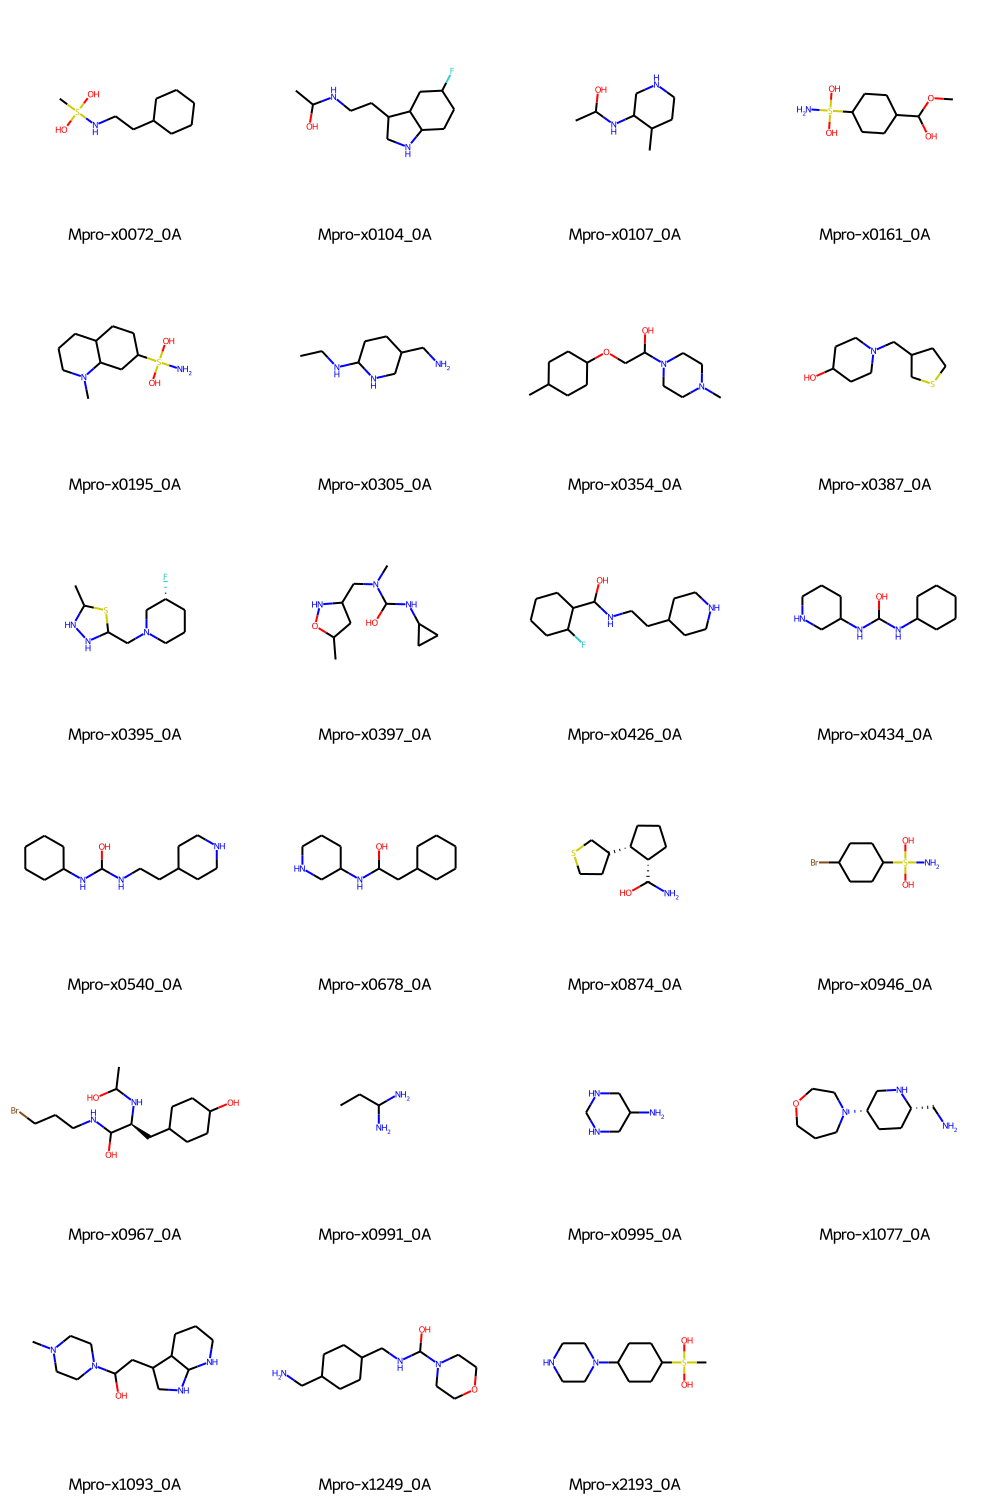
\includegraphics[width=0.8\textwidth]{paper/Figures/FigS1/mpro_ligands_grid_2d.png}
    \caption{2D Mpro structures from the moonshot dataset.}
    \label{fig:fragments}
\end{figure}
\newpage
\paragraph{Curated samples from different SILVR rates}
Figure~\ref{fig:fig_2} contains two examples started from fragments \texttt{xxx} and \texttt{xxx} and resulting samples for different SILVR rates $r_{\mathrm{S}}$.
\begin{figure}[hb!]
    \centering
    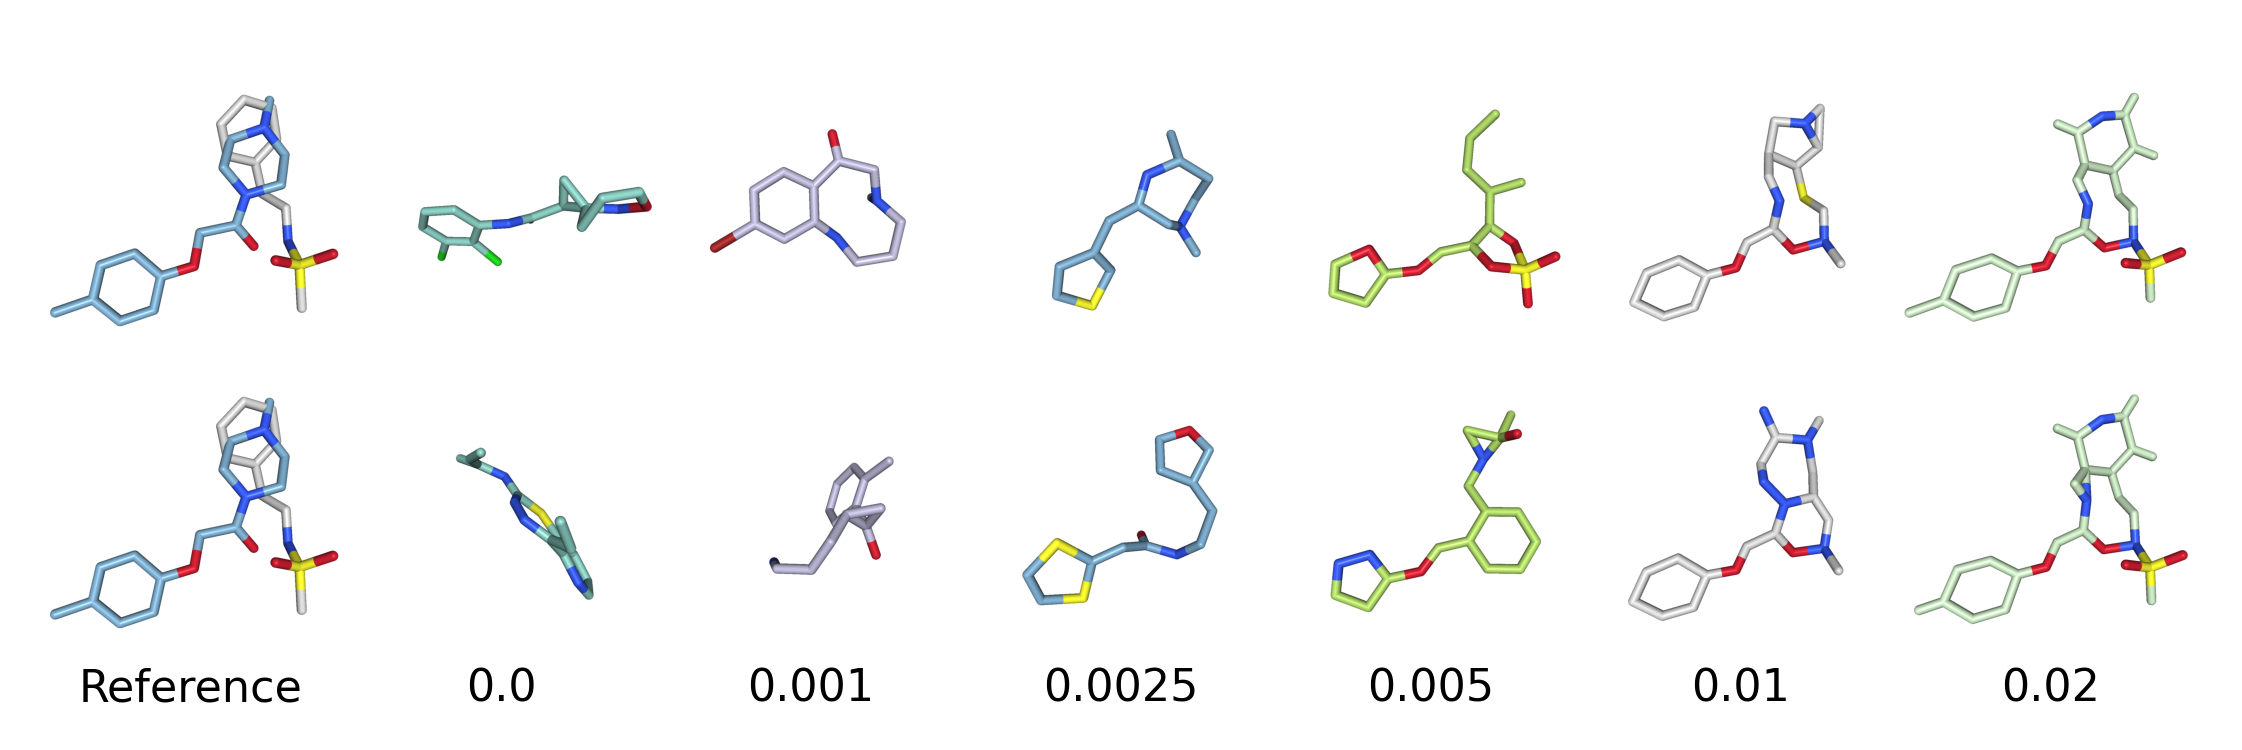
\includegraphics[width=\textwidth]{paper/Figures/FigS2/fig_2_sample_vs_rate.png}
    \caption{Two random samples from the same reference using different SILVR rates. All bonds were inferred from \texttt{XYZ} coordinates with OpenBabel. All bonds were visualised as single bonds and hydrogen atoms were deleted for clarity. Increasing SILVR rate results in sampled atom coordinates coming closer in space, and element type, to the reference while still resembling a truly molecular structure.}
    \label{fig:fig_2}
\end{figure}
\nemapge

\paragraph{Examples of uncurated samples}

\begin{figure}
    \centering
    \includegraphics{}
    \caption{Caption}
    \label{fig:my_label}
\end{figure}

\end{suppinfo}

\end{document}